\documentclass{standalone}
\usepackage{xcolor}
\usepackage{verbatim}
\usepackage[T1]{fontenc}
\usepackage{graphics}
\usepackage{hyperref}
\newcommand{\code}[1]{\texttt{#1}}
\newcommand{\R}{R}
\newcommand{\pkg}[1]{#1}
\newcommand{\CRANpkg}[1]{\pkg{#1}}%
\newcommand{\BIOpkg}[1]{\pkg{#1}}
\usepackage{amsmath,amssymb,array}
\usepackage{booktabs}
\usepackage[english]{babel}
\usepackage{subcaption}
\usepackage{amsfonts}
\usepackage{bbm}
\usepackage{tikz}
\usetikzlibrary{automata,positioning}
\usepackage{bm}
\newcommand\codeNew{\bgroup\@makeother\_\@makeother\~\@makeother\$\@codex}

\begin{document}
\nopagecolor
	\centering
	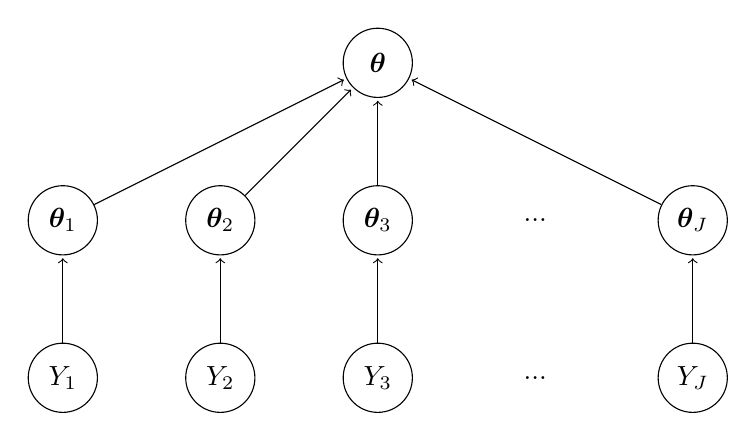
\begin{tikzpicture}[shorten >=1pt,node distance=2cm,on grid,auto]
	\node[state] (y1)  {$Y_1$}; 
	\node[state] (y2) [right=of y1] {$Y_2$}; 
	\node[state] (y3) [right=of y2] {$Y_3$}; 
	\node (dots) [right=of y3] {$...$}; 
	\node[state] (yk) [right=of dots] {$Y_J$}; 
	\node[state] (theta1) [above=of y1]  {${\bm\theta_1}$}; 
	\node[state] (theta2) [right=of theta1] {${\bm\theta_2}$}; 
	\node[state] (theta3) [right=of theta2] {${\bm\theta_3}$}; 
	\node (dots2) [right=of theta3] {$...$}; 
	\node[state] (thetak) [right=of dots2] {${\bm\theta_J}$}; 
	\node[state] (theta) [above=of theta3] {${\bm\theta}$};
	\path[->]
	(y1) edge node {} (theta1)
	(y2) edge node {} (theta2)
	(y3) edge node {} (theta3)
	(yk) edge node {} (thetak)
	(theta1) edge node {} (theta)
	(theta2) edge node {} (theta)
	(theta3) edge node {} (theta)
	(thetak) edge node {} (theta);
	\end{tikzpicture}
\end{document}
